% Figure 1: (a) the parts of a model prediction, from theory to predicted
% responses, and (b) the cycle of working with them. A standalone TikZ figure;
% from the Figures folder, pdflatex fig01_thinking_cycle.tex writes the PDF, and
% pdftoppm -r 300 -png -singlefile fig01_thinking_cycle.pdf fig01_thinking_cycle
% writes the PNG.
\documentclass[tikz,border=7pt]{standalone}
\usepackage[T1]{fontenc}
\usepackage{tgheros}
\renewcommand{\familydefault}{\sfdefault}
\usepackage{tikz}
\usetikzlibrary{arrows.meta,calc,positioning}

\definecolor{ink}{HTML}{1F2933}
\definecolor{muted}{HTML}{5F6B76}
\definecolor{hairline}{HTML}{BCC6CE}
\definecolor{panelrule}{HTML}{E3E8EC}
\definecolor{blue}{HTML}{315F7D}
\definecolor{bluefill}{HTML}{EDF4F8}

\newcommand{\main}[1]{{\bfseries\fontsize{8.3}{9.5}\selectfont #1}}
\newcommand{\sub}[1]{{\fontsize{7.0}{8.2}\selectfont\spaceskip=0.26em plus 0.08em minus 0.04em\relax\color{muted}#1}}
\newcommand{\step}[2]{{\bfseries\fontsize{8.4}{9.6}\selectfont\strut #1}\\[2.5pt]{\fontsize{7.0}{8.3}\selectfont\spaceskip=0.26em plus 0.08em minus 0.04em\relax\color{muted}#2\strut}}

\begin{document}
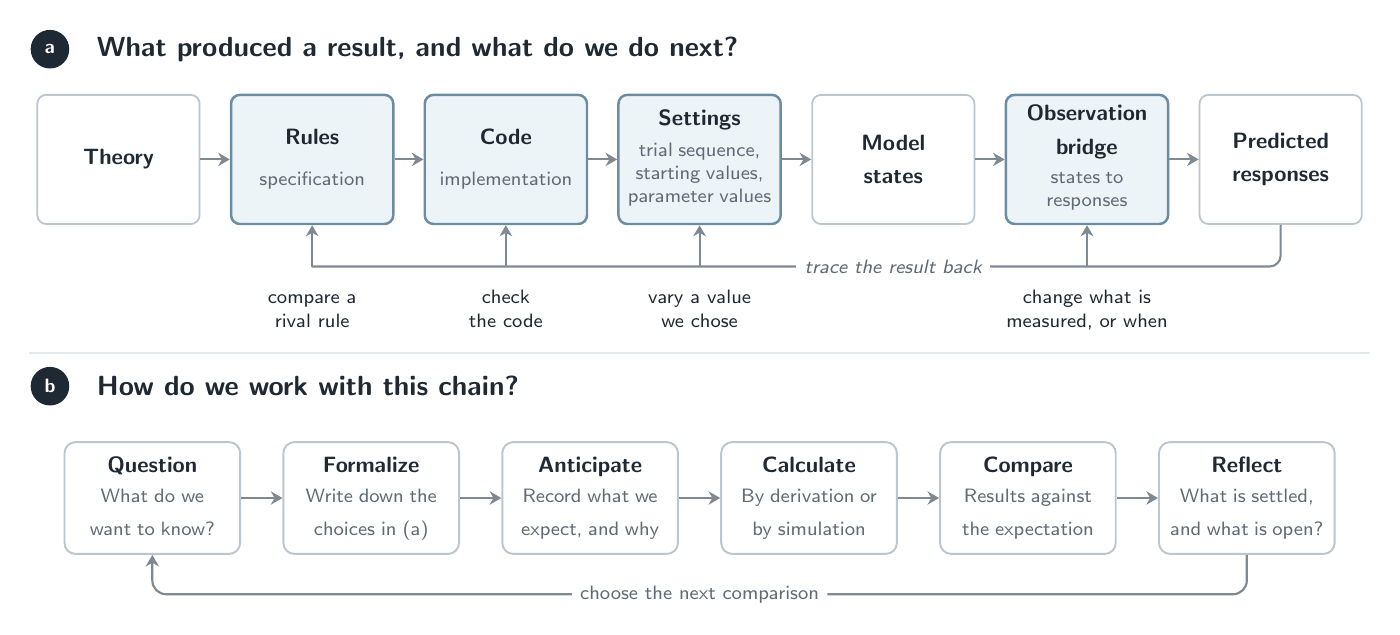
\begin{tikzpicture}[
  font=\sffamily,
  paneltitle/.style={anchor=west, font=\bfseries\fontsize{9.8}{11.2}\selectfont, text=ink},
  panellabel/.style={circle, fill=ink, text=white, minimum size=4.9mm, inner sep=0pt,
    font=\bfseries\fontsize{7.5}{8.3}\selectfont},
  chainbox/.style={draw=hairline, fill=white, rounded corners=3.2pt, line width=0.65pt,
    minimum width=2.0cm, minimum height=1.64cm, text width=1.92cm, inner sep=2pt, align=center, text=ink},
  choice/.style={chainbox, draw=blue!72, fill=bluefill, line width=0.9pt},
  chainarrow/.style={-{Stealth[length=4.2pt,width=4.8pt]}, draw=muted!80, line width=0.75pt},
  tracearrow/.style={-{Stealth[length=4.0pt,width=4.6pt]}, draw=muted!80, line width=0.75pt},
  nextstep/.style={align=center, anchor=north, font=\fontsize{7.2}{8.5}\selectfont, text=ink},
  workflow/.style={draw=hairline, fill=white, rounded corners=4pt, line width=0.7pt,
    minimum width=2.20cm, minimum height=1.42cm, text width=2.02cm, inner sep=3pt, align=center, text=ink},
  workflowarrow/.style={-{Stealth[length=4.2pt,width=4.8pt]}, draw=muted!80, line width=0.78pt}
]

% (a) What produced a result
\node[panellabel] (pa) at (-8.25,5.80) {a};
\node[paneltitle, right=2.2mm of pa] {What produced a result, and what do we do next?};

\node[chainbox] (theory) at (-7.38,4.40) {\main{Theory}};
\node[choice]   (spec)   at (-4.92,4.40) {\main{Rules}\\[3pt]\sub{specification}};
\node[choice]   (impl)   at (-2.46,4.40) {\main{Code}\\[3pt]\sub{implementation}};
\node[choice]   (set)    at (0,4.40)     {\main{Settings}\\[3pt]\sub{\begin{tabular}{@{}c@{}}trial sequence,\\starting values,\\parameter values\end{tabular}}};
\node[chainbox] (states) at (2.46,4.40)  {\main{Model\\states}};
\node[choice]   (bridge) at (4.92,4.40)  {\main{Observation\\bridge}\\[3pt]\sub{\begin{tabular}{@{}c@{}}states to\\responses\end{tabular}}};
\node[chainbox] (pred)   at (7.38,4.40)  {\main{Predicted\\responses}};
\foreach \a/\b in {theory/spec,spec/impl,impl/set,set/states,states/bridge,bridge/pred}
  \draw[chainarrow] (\a.east) -- (\b.west);

% tracing the result back: each choice points to a different next step
\draw[draw=muted!80, line width=0.75pt, rounded corners=4pt] (pred.south) |- (-4.92,3.04);
\foreach \n in {spec,impl,set,bridge} \draw[tracearrow] (\n.south |- 0,3.04) -- (\n.south);
\node[fill=white, inner xsep=3pt, inner ysep=1.5pt, font=\itshape\fontsize{7.2}{8.4}\selectfont, text=muted] at (2.46,3.04) {trace the result back};
\node[nextstep] at (-4.92,2.90) {\strut compare a\\rival rule};
\node[nextstep] at (-2.46,2.90) {\strut check\\the code};
\node[nextstep] at (0,2.90)     {\strut vary a value\\we chose};
\node[nextstep] at (4.92,2.90)  {\strut change what is\\measured, or when};

\draw[panelrule, line width=0.75pt] (-8.52,1.94) -- (8.52,1.94);

% (b) The cycle
\node[panellabel] (pb) at (-8.25,1.52) {b};
\node[paneltitle, right=2.2mm of pb] {How do we work with this chain?};

\node[workflow] (q) at (-6.95,0.10) {\step{Question}{What do we\\want to know?}};
\node[workflow] (f) at (-4.17,0.10) {\step{Formalize}{Write down the\\choices in (a)}};
\node[workflow] (a) at (-1.39,0.10) {\step{Anticipate}{Record what we\\expect, and why}};
\node[workflow] (s) at (1.39,0.10)  {\step{Calculate}{By derivation or\\by simulation}};
\node[workflow] (x) at (4.17,0.10)  {\step{Compare}{Results against\\the expectation}};
\node[workflow] (r) at (6.95,0.10)  {\step{Reflect}{What is settled,\\and what is open?}};
\foreach \a/\b in {q/f,f/a,a/s,s/x,x/r} \draw[workflowarrow] (\a.east) -- (\b.west);
\draw[workflowarrow, rounded corners=5pt] (r.south) -- ++(0,-0.50)
  -- node[midway, fill=white, inner xsep=3pt, inner ysep=1.5pt, font=\fontsize{7.0}{8.2}\selectfont, text=muted] {choose the next comparison}
  ($(q.south)+(0,-0.50)$) -- (q.south);
\end{tikzpicture}
\end{document}
